\documentclass[border=4pt,tikz]{standalone}
\usepackage[T1]{fontenc}
\usepackage{lmodern}
\usepackage{amsmath}
\usetikzlibrary{positioning,arrows.meta,calc,fit,backgrounds,patterns}
% Shared visual language for the paper's architecture diagrams.
% Every fill differs in lightness, so the diagrams stay legible when printed
% in grayscale; colour is only a redundant cue.
\definecolor{ink}{HTML}{1B2A3A}
\definecolor{navyfill}{HTML}{D5E0EC}
\definecolor{navyedge}{HTML}{2F5D8A}
\definecolor{tealfill}{HTML}{BFD8D5}
\definecolor{tealedge}{HTML}{2A6F6C}
\definecolor{amberfill}{HTML}{F1DCAE}
\definecolor{amberedge}{HTML}{9C6512}
\definecolor{greyfill}{HTML}{E5E7EB}
\definecolor{greymid}{HTML}{8B939E}
\definecolor{redfill}{HTML}{F0CBC5}
\definecolor{rededge}{HTML}{9E3B32}

\tikzset{
  >={Stealth[length=2.0mm,width=1.5mm]},
  every node/.style={font=\footnotesize, text=ink},
  box/.style={draw=ink, line width=0.5pt, rounded corners=1.5pt,
              fill=greyfill, align=center, inner sep=3pt, minimum height=7mm},
  databox/.style={box, fill=amberfill, draw=amberedge},
  procbox/.style={box, fill=navyfill, draw=navyedge},
  repbox/.style={box, fill=tealfill, draw=tealedge},
  evalbox/.style={box, fill=redfill, draw=rededge},
  fadebox/.style={box, fill=white, draw=greymid, dashed},
  arr/.style={->, draw=ink, line width=0.6pt},
  darr/.style={->, draw=greymid, line width=0.6pt, dashed},
  lbl/.style={font=\scriptsize, text=ink, inner sep=1pt, fill=white, fill opacity=0.85, text opacity=1},
  note/.style={font=\scriptsize, text=ink, align=left, inner sep=1pt},
  badge/.style={draw=rededge, fill=redfill, rounded corners=6pt,
                font=\scriptsize\bfseries, text=rededge, inner sep=2.2pt},
  badgefrz/.style={draw=tealedge, fill=tealfill, rounded corners=6pt,
                font=\scriptsize\bfseries, text=tealedge, inner sep=2.2pt},
  group/.style={draw=greymid, line width=0.5pt, rounded corners=3pt, inner sep=6pt},
}


% Schematic of the evaluation protocol. Curves are illustrative, not measured
% data; the caption says so. No result numbers are baked into this figure.
\begin{document}
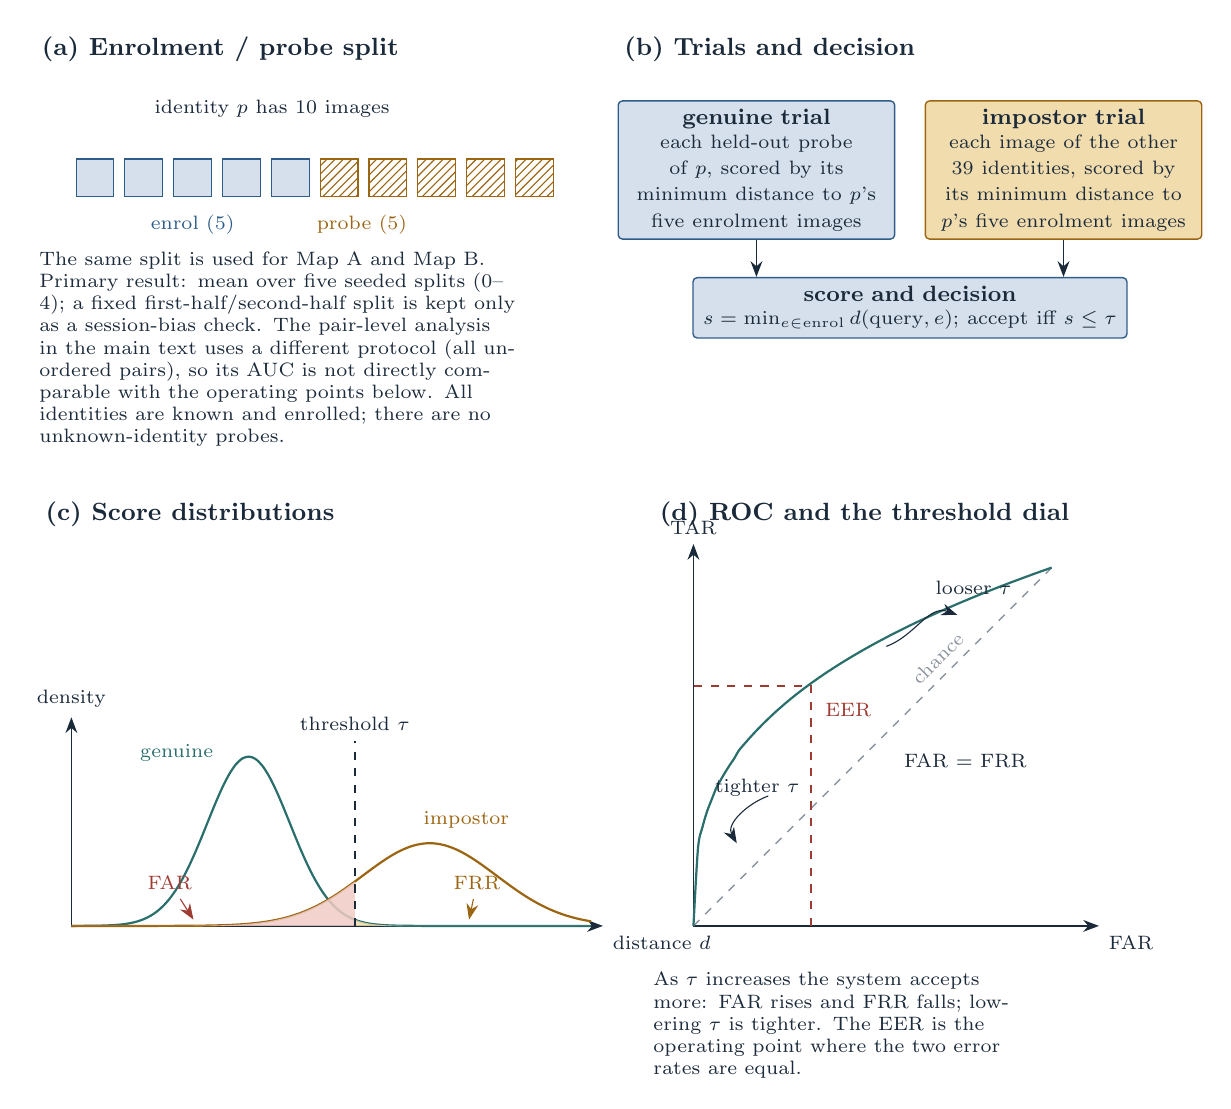
\begin{tikzpicture}[x=1cm,y=1cm]

% ============================================================= (a) split
\node[font=\small\bfseries, anchor=south west] at (0.15,7.55) {(a) Enrolment / probe split};
\node[font=\scriptsize, anchor=south] at (3.20,6.85) {identity $p$ has 10 images};
\foreach \i in {0,...,4} {
  \node[draw=navyedge, fill=navyfill, minimum size=0.48cm, inner sep=0pt] at (0.95+0.62*\i,6.20) {};
}
\foreach \i in {0,...,4} {
  \node[draw=amberedge, fill=amberfill, minimum size=0.48cm, inner sep=0pt, pattern=north east lines, pattern color=amberedge] at (4.05+0.62*\i,6.20) {};
}
\node[font=\scriptsize, text=navyedge, anchor=north] at (2.19,5.85) {enrol (5)};
\node[font=\scriptsize, text=amberedge, anchor=north] at (4.34,5.85) {probe (5)};

\node[note, anchor=north west, text width=6.2cm] at (0.20,5.30)
  {The same split is used for Map A and Map B. Primary result: mean over five seeded
   splits (0--4); a fixed first-half/second-half split is kept only as a session-bias check.
   The pair-level analysis in the main text uses a different protocol (all unordered pairs),
   so its AUC is not directly comparable with the operating points below. All identities are
   known and enrolled; there are no unknown-identity probes.};

% ============================================================= (b) trials
\node[font=\small\bfseries, anchor=south west] at (7.55,7.55) {(b) Trials and decision};
\node[procbox, text width=3.3cm] (gen) at (9.35,6.30)
  {\textbf{genuine trial}\\[-1pt] \scriptsize each held-out probe of $p$, scored by its minimum distance to $p$'s five enrolment images};
\node[databox, text width=3.3cm] (imp) at (13.25,6.30)
  {\textbf{impostor trial}\\[-1pt] \scriptsize each image of the other 39 identities, scored by its minimum distance to $p$'s five enrolment images};
\node[procbox, text width=5.3cm] (dec) at (11.30,4.55)
  {\textbf{score and decision}\\[-1pt] \scriptsize $s = \min_{e \in \mathrm{enrol}} d(\text{query}, e)$; accept iff $s \le \tau$};

\draw[arr] (gen.south) -- (gen.south |- dec.north);
\draw[arr] (imp.south) -- (imp.south |- dec.north);

% ============================================================= (c) distributions
\begin{scope}[shift={(0.65,-3.30)}]
  \node[font=\small\bfseries, anchor=south west] at (-0.45,4.95) {(c) Score distributions};
  \draw[->, draw=ink, line width=0.5pt] (0,0) -- (6.75,0) node[below right, font=\scriptsize] {distance $d$};
  \draw[->, draw=ink, line width=0.5pt] (0,0) -- (0,2.65) node[above, font=\scriptsize] {density};

  % genuine and impostor curves (illustrative shapes)
  \draw[thick, tealedge] plot[domain=0:6.6, smooth, samples=80] (\x, {2.15*exp(-((\x-2.25)^2)/0.55)});
  \draw[thick, amberedge] plot[domain=0:6.6, smooth, samples=80] (\x, {1.05*exp(-((\x-4.55)^2)/1.45)});

  % FAR = impostor mass at or below tau
  \fill[redfill, opacity=0.85] (0,0) -- plot[domain=0:3.60, smooth, samples=40] (\x, {1.05*exp(-((\x-4.55)^2)/1.45)}) -- (3.60,0) -- cycle;
  % FRR = genuine mass above tau
  \fill[amberfill, opacity=0.85] (3.60,0) -- plot[domain=3.60:6.6, smooth, samples=40] (\x, {2.15*exp(-((\x-2.25)^2)/0.55)}) -- (6.6,0) -- cycle;

  \draw[dashed, draw=ink, line width=0.7pt] (3.60,0) -- (3.60,2.35) node[above, font=\scriptsize] {threshold $\tau$};

  \node[font=\scriptsize, text=rededge] (far) at (1.25,0.55) {FAR};
  \node[font=\scriptsize, text=amberedge] (frr) at (5.15,0.55) {FRR};
  \node[font=\scriptsize, text=tealedge, anchor=west] at (0.75,2.20) {genuine};
  \node[font=\scriptsize, text=amberedge, anchor=west] at (4.35,1.35) {impostor};
  \draw[->, draw=rededge, line width=0.4pt] (far) -- (1.55,0.08);
  \draw[->, draw=amberedge, line width=0.4pt] (frr) -- (5.05,0.08);
\end{scope}

% ============================================================= (d) ROC
\begin{scope}[shift={(8.55,-3.30)}]
  \node[font=\small\bfseries, anchor=south west] at (-0.55,4.95) {(d) ROC and the threshold dial};
  \draw[->, draw=ink, line width=0.5pt] (0,0) -- (5.15,0) node[below right, font=\scriptsize] {FAR};
  \draw[->, draw=ink, line width=0.5pt] (0,0) -- (0,4.85) node[above, font=\scriptsize] {TAR};

  % chance line and one operating curve (illustrative)
  \draw[dashed, draw=greymid, line width=0.5pt] (0,0) -- (4.55,4.55);
  \node[font=\scriptsize, text=greymid, rotate=45, anchor=south] at (3.25,3.25) {chance};
  \draw[thick, tealedge] plot[domain=0:4.55, smooth, samples=80] (\x, {4.55*(\x/4.55)^0.35});

  % EER point: FAR = FRR where TAR = 1 - FAR
  \coordinate (eer) at (1.49,3.05);
  \draw[dashed, draw=rededge, line width=0.6pt] (1.49,0) -- (1.49,3.05) -- (0,3.05);
  \node[font=\scriptsize, text=rededge, anchor=north west] at (1.55,2.95) {EER};
  \node[font=\scriptsize, text=ink, anchor=west] at (2.55,2.10) {FAR = FRR};

  % threshold direction along the curve
  \node[font=\scriptsize, text=ink, anchor=west] at (2.95,4.30) {looser $\tau$};
  \draw[->, draw=ink, line width=0.4pt] (2.45,3.55) to[out=20,in=160] (3.35,3.95);
  \node[font=\scriptsize, text=ink, anchor=west] at (0.15,1.75) {tighter $\tau$};
  \draw[->, draw=ink, line width=0.4pt] (0.95,1.65) to[out=200,in=120] (0.55,1.05);

  \node[note, anchor=north west, text width=4.6cm] at (-0.55,-0.55)
    {As $\tau$ increases the system accepts more: FAR rises and FRR falls; lowering $\tau$ is
     tighter. The EER is the operating point where the two error rates are equal.};
\end{scope}

\end{tikzpicture}
\end{document}
